\documentclass[hidelinks,12pt]{article}
\usepackage[left=0.25cm,top=1cm,right=0.25cm,bottom=1cm]{geometry}
%\usepackage[landscape]{geometry}
\textwidth = 20cm
\hoffset = -1cm
\usepackage[utf8]{inputenc}
\usepackage[spanish,es-tabla]{babel}
\usepackage[autostyle,spanish=mexican]{csquotes}
\usepackage[tbtags]{amsmath}
\usepackage{nccmath}
\usepackage{amsthm}
\usepackage{amssymb}
\usepackage{mathrsfs}
\usepackage{graphicx}
\usepackage{subfig}
\usepackage{standalone}
\usepackage[outdir=./Imagenes/]{epstopdf}
\usepackage{siunitx}
\usepackage{physics}
\usepackage{color}
\usepackage{float}
\usepackage{hyperref}
\usepackage{multicol}
%\usepackage{milista}
\usepackage{anyfontsize}
\usepackage{anysize}
%\usepackage{enumerate}
\usepackage[shortlabels]{enumitem}
\usepackage{capt-of}
\usepackage{bm}
\usepackage{relsize}
\usepackage{placeins}
\usepackage{empheq}
\usepackage{cancel}
\usepackage{wrapfig}
\usepackage[flushleft]{threeparttable}
\usepackage{makecell}
\usepackage{fancyhdr}
\usepackage{tikz}
\usepackage{bigints}
\usepackage{scalerel}
\usepackage{pgfplots}
\usepackage{pdflscape}
\pgfplotsset{compat=1.16}
\spanishdecimal{.}
\renewcommand{\baselinestretch}{1.5} 
\renewcommand\labelenumii{\theenumi.{\arabic{enumii}})}
\newcommand{\ptilde}[1]{\ensuremath{{#1}^{\prime}}}
\newcommand{\stilde}[1]{\ensuremath{{#1}^{\prime \prime}}}
\newcommand{\ttilde}[1]{\ensuremath{{#1}^{\prime \prime \prime}}}
\newcommand{\ntilde}[2]{\ensuremath{{#1}^{(#2)}}}

\newtheorem{defi}{{\it Definición}}[section]
\newtheorem{teo}{{\it Teorema}}[section]
\newtheorem{ejemplo}{{\it Ejemplo}}[section]
\newtheorem{propiedad}{{\it Propiedad}}[section]
\newtheorem{lema}{{\it Lema}}[section]
\newtheorem{cor}{Corolario}
\newtheorem{ejer}{Ejercicio}[section]

\newlist{milista}{enumerate}{2}
\setlist[milista,1]{label=\arabic*)}
\setlist[milista,2]{label=\arabic{milistai}.\arabic*)}
\newlength{\depthofsumsign}
\setlength{\depthofsumsign}{\depthof{$\sum$}}
\newcommand{\nsum}[1][1.4]{% only for \displaystyle
    \mathop{%
        \raisebox
            {-#1\depthofsumsign+1\depthofsumsign}
            {\scalebox
                {#1}
                {$\displaystyle\sum$}%
            }
    }
}
\def\scaleint#1{\vcenter{\hbox{\scaleto[3ex]{\displaystyle\int}{#1}}}}
\def\bs{\mkern-12mu}


%\usepackage{showframe}
\usepackage{apacite}
\title{Funciones Asociadas de Legendre \\ \large {Tema 4 - Sep. variables en coord. esféricas} \vspace{-3ex}}
\author{M. en C. Gustavo Contreras Mayén}
\date{ }
\begin{document}
\vspace{-4cm}
\maketitle
\fontsize{14}{14}\selectfont
\tableofcontents
\newpage
\section{Funciones asociadas de Legendre.}
La ecuación asociada de Legendre tiene la forma
\begin{align}
(1 - x^{2}) \, \stilde{y} - 2 \, x \, \ptilde{y} + \left[ \ell (\ell + 1) - \dfrac{m^{2}}{1 - x^{2}} \right] \, y = 0
\label{eq:ecuacion_18_28}
\end{align}
que tiene tres puntos singulares en $x = -1, 1, \infty$, se reduce a la ecuación de Legendre cuando $m=0$, vista en el material anterior.
\par
Se presenta en problemas de la física que involucran el operador $\nabla^{2}$, cuando se expresa en coordenadas polares. En esos casos, $- \ell \leq m \leq \ell$ y $m$ está restringida a valores enteros.
\par
Como en el caso de la ecuación de Legendre, la variable $x$ es el coseno del ángulo polar en coordenadas esféricas, por tanto $-1 \leq x \leq 1$. Cualquier solución de la ecuación \ref{eq:ecuacion_18_28}) es llamada la \emph{función asociada de Legendre}.
\par
El punto $x = 0$ es un punto ordinario, y del cual se pueden obtener soluciones en series de la forma
\begin{align*}
y = \sum_{n=0} a_{n} \, x^{n}
\end{align*}
de la misma manera que se hizo para la ecuación de Legendre. En este caso, debemos de notar que si $u(x)$ es solución de la ecuación de Legendre, entonces
\begin{align}
y(x) = (1 -x^{2})^{\abs{m}/2} \dv[\abs{m}]{u}{x}
\label{eq:ecuacion_18_29}
\end{align}
es solución a la ecuación asociada (\ref{eq:ecuacion_18_28}).
\par
Veamos que si $u(x)$ es solución de la ecuación de Legendre, entonces $y(x)$ dada por la ec. (\ref{eq:ecuacion_18_29}) es una solución a la ecuación asociada de Legendre:
\par
Por simplificidad, consideremos que $m$ no es negativo, la ecuación de Legendre para $u$ es:
\begin{align*}
(1 - x^{2}) \, \stilde{y} - 2 \, x \, \ptilde{y} + \left[ \ell (\ell + 1) \right] \, y = 0
\end{align*}
al diferenciar $m$ veces esta ecuación mediante el teorema de Leibinz, obtenemos:
\begin{align}
(1 - x^{2}) \, \stilde{v} - 2 \, x \, (m + 1) \, \ptilde{v} + \left[ \ell - m) (\ell + m + 1) \right] \, v = 0
\label{eq:ecuacion_18_30}
\end{align}
donde $v(x) = \dv*[m]{u}{x}$.
\par
Definiendo:
\begin{align*}
y(x) = (1 - x^{2}) ^{m/2} \, v(x)
\end{align*}
Las derivadas de $\ptilde{v}$ y $\stilde{v}$ se pueden escribir como
\begin{align*}
\ptilde{v} &= (1 - x^{2})^{-m/2} \, \left( \ptilde{y} + \dfrac{m \, x}{1 -x^{2}} \, y \right) \\[1em]
\stilde{v} &= (1 - x^{2})^{-m/2} \, \left[ \stilde{y} + \dfrac{2 \, m \, x}{1 -x^{2}} \, \ptilde{y} + \dfrac{m \, x}{1 -x^{2}} \, y + \dfrac{m(m + 2) \, x^{2}}{(1 -x^{2})^{2}} \, y \right]
\end{align*}
Sustituyendo las expresiones en la ec. (\ref{eq:ecuacion_18_30}), para luego simplificar llegamos a:
\begin{align*}
(1 - x^{2}) \, \stilde{y} - 2 \, x \, \ptilde{y} + \left[ \ell (\ell + 1) - \dfrac{m^{2}}{1 - x^{2}} \right] \, y = 0
\end{align*}
lo que demuestra que $y$ es solución a la ecuación asociada de Legendre (\ref{eq:ecuacion_18_28}). En caso de que $m$ sea negativo, el valor de $m^{2}$ no se modifica, por lo que una solución para $m$ positivo, es también una solución para el correspondiente valor de $m$ negativo.
\par
De las dos soluciones en serie linealmente independientes de la ecuación de Legendre dada por:
\begin{align*}
y_{1}(x) &= 1 - \ell (\ell + 1) \dfrac{x^{2}}{2!} + (\ell - 2)\; \ell \; (\ell + 1)\;(\ell + 3) \dfrac{x^{4}}{4!} - \ldots \\[1em]
y_{2}(x) &= x - (\ell - 1)(\ell + 2) \dfrac{x^{3}}{3!} + (\ell - 3) (\ell - 1)(\ell + 2)(\ell + 4) \dfrac{x^{5}}{5!} - \ldots
\end{align*}
que ahora denotamos por $u_{1} (x)$ y $u_{2}(x)$, podemos obtener dos soluciones en serie linealmente independientes, $y_{1} (x)$ y $y_{2} (x)$, a la ecuación asociada de Legendre mediante el uso de (\ref{eq:ecuacion_18_29}). A partir de la discusión general de la convergencia de la serie de potencias, vemos que ambas $y_{1} (x)$ y $y_{2} (x)$ también convergen para $\abs{x} < 1$. Por lo tanto la solución general de la ecuación(\ref{eq:ecuacion_18_28}) en este rango está dado por
\begin{align*}
y(x) = c_{1} \, y_{1} (x) + c_{2} \, y_{2} (x)
\end{align*}
\subsection{Funciones asociadas de Legendre para enteros $\ell$.}
Si $\ell$ y $m$ son ambos enteros, como en el caso de varios problemas de la física, entonces la solución general de la ecuación (\ref{eq:ecuacion_18_28}) se expresa por
\begin{align}
y(x) = c_{1} \, P_{\ell}^{m} (x) + c_{2} \, Q_{\ell}^{m} (x)
\label{eq:ecuacion_18_31}
\end{align}
donde $P_{\ell}^{m} (x)$ y $Q_{\ell}^{m} (x)$ son las funciones asociadas de Legendre de primera y segunda clase, respectivamente. Para valores no negativos de $m$, esas funciones están relacionadas a las funciones de Legendre para enteros $\ell$ mediante
\begin{align}
\begin{aligned}
P_{\ell}^{m} (x) &= (1 - x^{2})^{m/2} \dv[m]{P_{\ell}}{x}, \\[1em]
Q_{\ell}^{m} (x) &= (1 - x^{2})^{m/2} \dv[m]{Q_{\ell}}{x}
\end{aligned}
\label{eq:ecuacion_18_32}
\end{align}
Vemos inmediatamente que, en caso necesario, las funciones asociadas de Legendre se reducen a las funciones ordinarias de Legendre cuando $m = 0$. 
\par
Dado que $m^{2}$ aparece en la ecuación asociada de Legendre -ec. (\ref{eq:ecuacion_18_28})-, las funciones asociadas de Legendre para los valores negativos $m$ debe ser proporcional a la función correspondiente para valores no negativos $m$. La constante de proporcionalidad es una cuestión de convención. Para el $P_{\ell}^{m} (x) $, es habitual considerar la definición (\ref{eq:ecuacion_18_32}) como válida también para los valores negativos $m$. Aunque la diferenciación de un número negativo no está definida, cuando $P_{\ell}(x)$ se expresa en términos de la fórmula de Rodrigues (de los polinomios de Legendre), este problema no se presenta para $\ell \leq m \leq \ell$. En este caso,
\begin{align}
P_{\ell}^{-m} (x) = (-1)^{m} \; \dfrac{(\ell - m)!}{(\ell + m)!} \, P_{\ell}^{m} (x)
\label{eq:ecuacion_18_33}
\end{align}
Ya que $P_{\ell}(x)$ es un polinomio de orden $\ell$, tenemos que $P_{\ell}^{m}(x)=0$ para $\abs{m} > \ell$. De esta definición, queda claro que $P_{\ell}^{m} (x)$ es también un polinomio de orden $\ell$ si $m$ es par, ya que contiene el factor $(1-x^{2})$ a una potencial fraccionaria si $m$ es impar. En cualquier caso $P_{\ell}^{m}(x)$ es regular en $x = \pm 1$.
\par
Los primeros polinomios asociados de Legendre de primera clase, se construyen fácilmente y están dadas por (se omiten los casos $m=0$):
\begin{align*}
P_{1}^{1} (x) &= (1 - x^{2})^{1/2} \\[0.5em]
P_{2}^{1} (x) &= 3 \, x \, (1 - x^{2})^{1/2} \\[0.5em]
P_{2}^{2} (x) &= 3 \, (1 - x^{2}) \\[0.5em]
P_{3}^{1} (x) &= \dfrac{3}{2}(5 \, x^{2} - 1)(1 - x^{2})^{1/2} \\[0.5em]
P_{3}^{2} (x) &= 15 \, x (1 - x^{2}) \\[0.5em]
P_{3}^{3} (x) &= 15 \, (1 - x^{2})^{3/2}
\end{align*}
\begin{figure}[H]
    \centering
    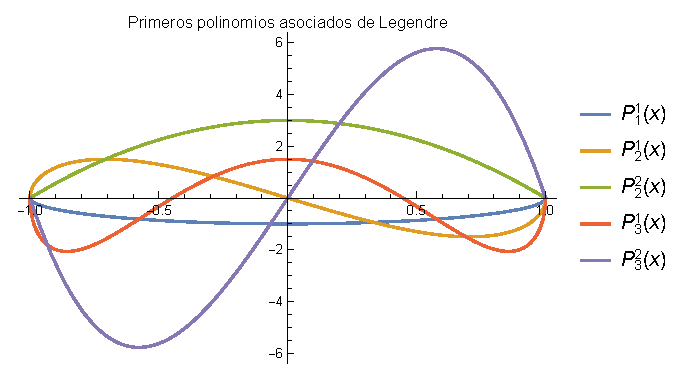
\includegraphics[scale=1]{Imagenes/Plot_Asociados_Lagrange.eps}
    \caption{Gráfica de los primeros polinomios asociados de Legendre, no se incluyen aquellos con $m = 0$.}
    \label{fig:figura_asociados_Legedre}
\end{figure}
Debemos de mencionar que las funciones asociadas de Legendre de segunda clase $Q_{\ell}^{m} (x)$ como las $Q_{\ell}(x)$ son singulares en $x = \pm 1$.
\subsection{Propiedades de las funciones asociadas de Legendre $P_{\ell}^{m}$.}
Cuando encontramos en problemas físicos, la variable $x$ de la ecuación asociada de Legendre (como en la ecuación ordinaria Legendre) es generalmente el coseno del ángulo polar $\theta$ en coordenadas polares esféricas, y entonces queremos que la solución $y (x)$ sea regular en $x = \pm 1$ (correspondiente a $\theta = 0$ o $\theta = \pi$). Para que esto ocurra, se requiere que $\ell$ sea un número entero y que el coeficiente $c_{2}$ de la función $Q_{\ell}^{m} (x)$ en la ecuación (\ref{eq:ecuacion_18_31}) sea cero, dado que $Q_{\ell}^{m}(x)$ es singular en $x = \pm 1$, con el resultado de que la solución general son múltiplos de las funciones asociadas de Legendre de primera clase $P_{\ell}^{m}(x)$.
\subsection{Ortogonalidad mutua.}
Ya se mencionó anteriormente que la ecuación asociada de Legendre es del tipo Sturm-Liouville de la forma
\begin{align*}
\ptilde{(p \, y)} + q \, y + \lambda \,  \omega \, y = 0
\end{align*}
con
\begin{align*}
p &= 1 - x^{2} \\[0.5em]
q &= - \dfrac{m^{2}}{(1 - x^{2})} \\[0.5em]
\lambda &= \ell (\ell + 1) \\[0.5em]
\omega &= 1
\end{align*}
siendo su intervalo natural en $[-1,1]$.
\par
Dado que las funciones asociadas de Legendre $P_{\ell}^{m} (x)$ son regulares en los extremos $x = \pm 1$, entonces deben de ser mutuamente ortogonales en este intervalo para un valor fijo de $m$, es decir:
\begin{align}
\int_{-1}^{1} P_{\ell}^{m} (x) \, P_{k}^{m} (x) \dd{x}  = 0, \hspace{1cm} \mbox{ si } \ell \neq	 k
\label{eq:ecuacion_18_36}
\end{align}
Nótese que el valor de $m$ debe de ser el mismo en ambas funciones asociadas de Legendre para que la expresión sea válida. La condición de normalización cuando $\ell = k$ se obtiene de la fórmula de Rodrigues:
\begin{align}
I_{\ell m} = \int_{-1}^{1} P_{\ell}^{m} (x) \, P_{\ell}^{m} (x) \dd{x} = \dfrac{2}{2 \, \ell + 1} \, \dfrac{(\ell + m)!}{( \ell - m)!}
\label{eq:ecuacion_18_37}
\end{align}
Las condiciones de ortogonalidad y normalización, ecuaciones (\ref{eq:ecuacion_18_36}) y (\ref{eq:ecuacion_18_37}), respectivamente, significan que los polinomios asociados de Legendre $P_{\ell}^{m}(x)$, con $m$ fija, puede utilizarse de manera similar a los polinomios de Legendre para expandir cualquier función $f(x)$ razonable en el intervalo $\abs{x} < 1$ en una serie de la forma
\begin{align}
f(x) = \sum_{k=0}^{\infty} a_{m+k} \, P_{m+k}^{m} (x)
\label{eq:ecuacion_18_38}
\end{align}
donde los coeficientes están dado por
\begin{align*}
a_{\ell} = \dfrac{2 \, \ell + 1}{2} \, \dfrac{(\ell - m)!}{(\ell + m)!} \int_{-1}^{1} f(x) \, P_{\ell}^{m} (x) \dd{x}
\end{align*}
\subsection{Función generatriz.}
La función generatriz para las funciones asociadas de Legendre, se obtienen de la combinación de su definición con la función generatriz de los polinomios de Legendre:
\begin{align}
G(x, h) = \dfrac{(2 \, m)(1 - x^{2})^{m/2}}{2^{m} \, m! \, (1 - 2 \, h \, x + h^{2})^{m+1/2}} = \sum_{n=0}^{\infty} P_{n+m}^{m} (x) \, h^{n}
\label{eq:ecuacion_18_40}
\end{align}
\subsection{Relaciones de recurrencia.}
Como era de esperar, las funciones asociadas de Legendre satisfacen ciertas relaciones de recurrencia. De hecho, la presencia de los dos índices $n$ y $m$ significa que se puede derivar una gama mucho más amplia de relaciones de recurrencia. Presentaremos sólo cuatro de las relaciones más útiles:
\begin{align*}
P_{n}^{m+1} &= \dfrac{2 \, m \, x}{(1 - x^{2})^{1/2}} P_{n}^{m} + [m (m - 1) - n (n + 1)] \, P_{n}^{m-1} \\[0.5em]
(2 \, n + 1) \, x \, P_{n}^{m} &= (n + m) \, P_{n-1}^{m} + (n - m + 1) \, P_{n+1}^{m} \\[0.5em]
(2 \, n + 1)(1 -  x^{2})^{1/2} P_{n}^{m} &= P_{n+1}^{m+1} - P_{n-1}^{m+1} \\[0.5em]
2 \, (1 - x^{2})^{1/2} \ptilde{(P_{n}^{m})} &= P_{n}^{m+1} - (n + m)(n - m + 1) \, P_{n}^{m-1}
\end{align*}
Las relaciones de recurrencia son válidas tanto para valores negativos como positivos de $m$.
\section{Armónicos esféricos.}
Las funciones asociadas de Legendre discutidas anteriormente se presentan más comúnmente la solución de la ecuación de Laplace $\laplacian =0$ en coordenadas polares esféricas. En particular, se encuentra que para las soluciones que son finitas en el eje polar, la parte angular de la solución viene dada por
\begin{align*}
\Theta (\theta) \, \Phi (\phi) = P_{\ell}^{m} (\cos \theta) \, (C \,  \cos m \phi + D \, \sin m \phi)
\end{align*}
donde $\ell$ y $m$ son enteros con $- \ell \leq m \leq \ell$. Esta forma general es muy común para funciones particulares de $\theta$ y $\phi$, se les llama \emph{armónicos esféricos}, se definen por
\begin{align}
Y_{\ell}^{m} (\theta, \phi) = (1-)^{m} \left[ \dfrac{2 \ell + 1}{4 \, \pi} \: \dfrac{(\ell + m)!}{(\ell - m)!} \right]^{1/2} \, P_{\ell}^{m} (\cos \theta) \exp(i \, m \, \phi)
\label{eq:ecuacion_18_45}
\end{align}
Usando la ecuación (\ref{eq:ecuacion_18_33}), encontramos que:
\begin{align*}
Y_{\ell}^{-m} (\theta, \phi) =  (-1)^{m} \left[ Y_{\ell}^{m} (\theta,\phi) \right]^{*}
\end{align*}
donde el asterisco indica el complejo conjugado. Los primeros armónicos esféricos $Y_{\ell}^{m}(\theta,\phi) \equiv Y_{\ell}^{m}$ son:
\begin{align*}
Y_{0}^{0} &= \sqrt{\dfrac{1}{4 \, \pi}} \\[0.5em]
Y_{1}^{0} &= \sqrt{\dfrac{3}{4 \, \pi}} \cos \theta \\[0.5em]
Y_{1}^{\pm 1} &= \mp \sqrt{\dfrac{3}{8 \, \pi}} \sin \theta \exp(\pm i \, \phi) \\[0.5em]
Y_{2}^{0} &= \sqrt{\dfrac{5}{16 \, \pi}} ( 3 \, \cos^{2} \theta - 1) \\[0.5em]
Y_{2}^{\pm 1} &= \mp \sqrt{\dfrac{15}{8 \, \pi}} \sin \theta \, \cos \theta \exp(\pm i \, \phi) \\[0.5em]
Y_{2}^{\pm 2} &= \sqrt{\dfrac{15}{32 \, \pi}} \sin^{2} \theta \exp(\pm 2 \, i \, \phi)
\end{align*}
Estas funciones se pueden visualizar haciendo una graficación en coordenadas polares en tres dimensiones de 
\begin{align*}
\abs{Y_{\ell}^{m} (\theta, \phi)}^{2} \hspace{0.2cm} \mbox{ contra } \theta \mbox{ y } \phi
\end{align*}
La gráfica para $Y_{0}^{0} (\theta, \phi)$ se muestra en la figura (\ref{fig:armonico_esferico_00}), donde la magnitud al cuadrado del armónico esférico está representado por la distancia del origen a la superficie.
\begin{figure}[H]
    \centering
    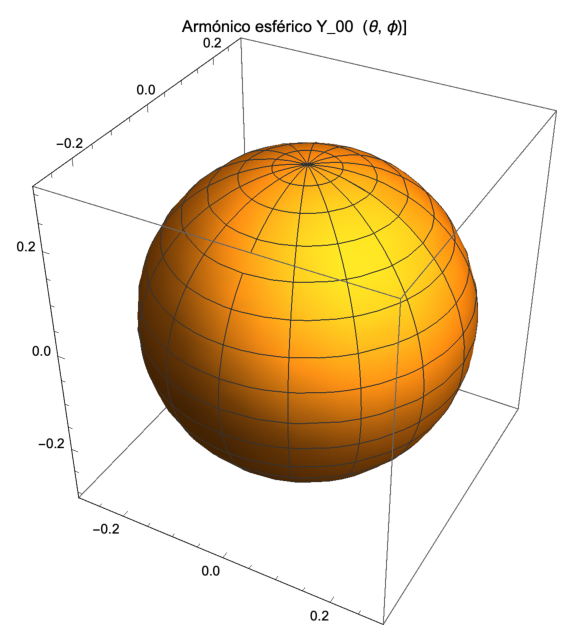
\includegraphics[scale=1]{Imagenes/Armonicos_Esfericos_00.eps}
    \label{fig:armonico_esferico_00}
\end{figure}
Las superficies similares se muestran para los armónicos esféricos $\ell = 1$ y $\ell = 2$; en éstas figuras, el eje $z$ es vertical, y las superficies son siempre simétricas sobre el eje, ya que $\abs{\exp(i \, m \, \phi)} = 1$. Por tanto, las gráficas para $\pm m$ son siempre las mismas, ya que
\begin{align*}
\abs{Y_{\ell}^{m}} = \abs{Y_{\ell}^{-m}}
\end{align*}

\begin{minipage}{0.4\textwidth}
    \centering
    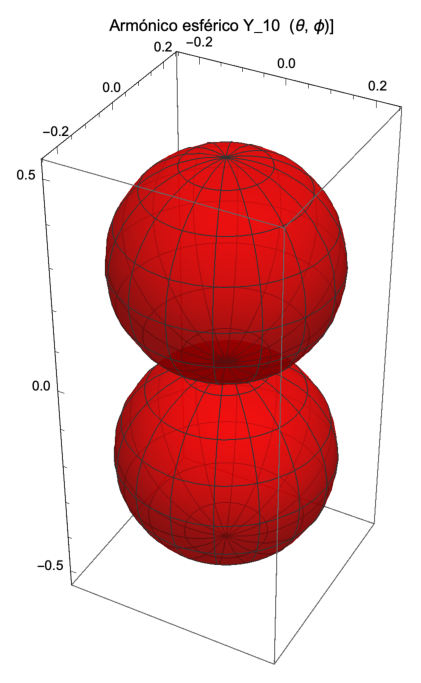
\includegraphics[scale=0.7]{Imagenes/Armonicos_Esfericos_10.eps}
\end{minipage}
\hspace{0.6cm}
\begin{minipage}{0.4\textwidth}
    \centering
    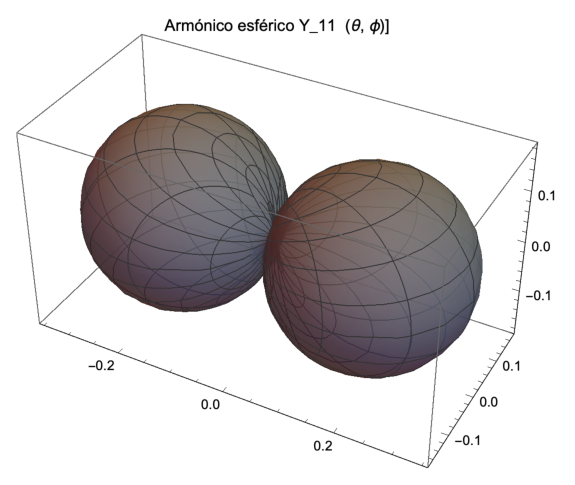
\includegraphics[scale=0.65]{Imagenes/Armonicos_Esfericos_11.eps}
\end{minipage}
\\[1em]
\begin{minipage}{0.4\textwidth}
    \centering
    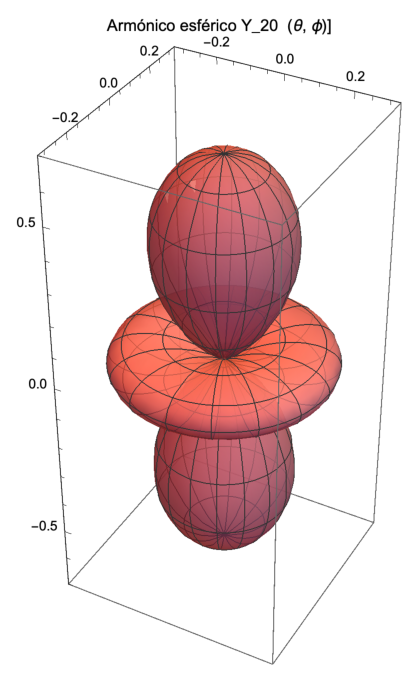
\includegraphics[scale=0.7]{Imagenes/Armonicos_Esfericos_20.eps}
\end{minipage}
\hspace{0.6cm}
\begin{minipage}{0.4\textwidth}
    \centering
    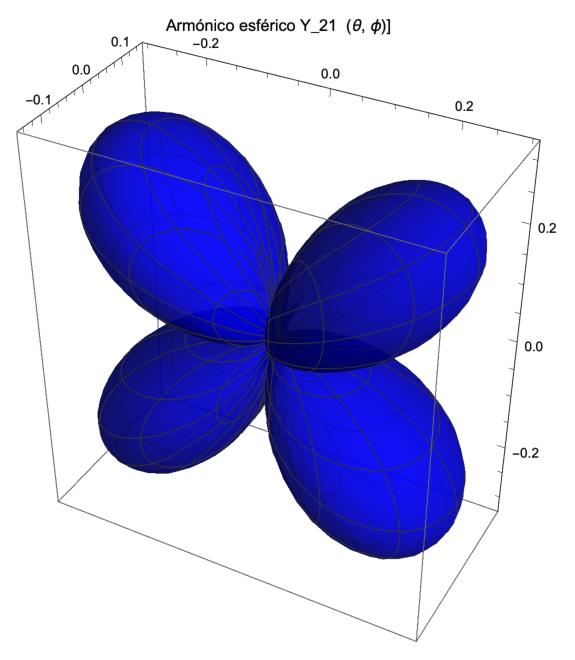
\includegraphics[scale=0.65]{Imagenes/Armonicos_Esfericos_21.eps}
\end{minipage}
\subsection{Ortogonalidad mutua.}
Ya que contienen su parte $\theta$-dependiente de la solución $P_{\ell}^{m}$ a la ecuación asociada de Legendre, el $Y_{\ell}^{m}$ son mutuamente ortogonales cuando se integra de $-1$ a $+1$ sobre $\dd{cos \theta}$.
\par
Su ortogonalidad mutua respecto de $\phi \, (0 \leq \phi \leq 2 \pi)$ es aún más evidente. El factor numérico en la ecuación (\ref{eq:ecuacion_18_45}) es elegido para hacer el $Y_{\ell}^{m}$ un conjunto ortonormal, es decir
\begin{align}
\int_{-1}^{1} \int_{0}^{2 \pi} [ Y_{\ell}^{m} (\theta, \phi) ]^{*} Y_{\ptilde{\ell}}^{\ptilde{m}} (\theta, \phi) \dd{\phi} \dd{(\cos \theta)} = \delta_{\ell \ptilde{\ell}} \,  \delta_{m \ptilde{m}}
\label{eq:ecuacion_18_46}
\end{align}
Adicionalmente, los armónicos esféricos forman un conjunto completo para cualquier función razonable de $\theta$ y $\phi$(como las que podemos encontrar en un problema físico), la función puede expandirse como una suma de tales funciones
\begin{align}
f(\theta, \phi) = \sum_{\ell=0}^{\infty} \sum_{-\ell}^{\ell} a_{\ell m} \, Y_{\ell}^{m} (\theta, \phi)
\label{eq:ecuacion_18_47}
\end{align}
las constantes $a_{\ell m}$ están dadas por
\begin{align}
a_{\ell m} = \int_{-1}^{1} \int_{0}^{2 \pi} [ Y_{\ell}^{m} (\theta, \phi) ]^{*} f (\theta, \phi) \dd{\theta} \dd{(\cos \theta)}
\label{eq:ecuacion_048}
\end{align}
Esto es una analogía exacta con una serie de Fourier y es un ejemplo particular de la propiedad general de soluciones de Sturm-Liouville.
\subsection{Teorema del desarrollo.}
Parte de la importancia de los armónicos esféricos se encuentra en la propiedad de completez, una consencuencia de la forma de Sturm-Liouville de la ecuación de Laplace.
\par
Esta propiedad, en este caso, significa que cualquier función $f(\theta, \phi)$, con las suficientes propiedades de continuidad, evaluada sobre la superficie de una esfera se puede desarrollar en una serie convergente de manera uniforme en los armónicos esféricos, que se le conoce como \emph{Serie de Laplace}:
\begin{align}
f(\theta, \phi) = \sum_{m, \ell} a_{m \ell} \, Y_{\ell}^{m} (\theta, \phi)
\label{eq:ecuacion_12_151}
\end{align}
Si $f(\theta, \phi)$ es conocida, los coeficientes se pueden encontrar de inmediato mediante el uso de la integral de ortogonalidad:
\begin{align}
a_{m \ell} = \int f(\theta, \phi) \, (Y_{\ell}^{m})^{*} (\theta, \phi) \dd{\Omega}
\label{eq:ecuacion_10_237}
\end{align}
donde $\dd{\Omega}$ es el elemento de ángulo sólido de la esfera.
\par
Haciendo un cambio de variable, es posible demostrar que:
\begin{align}
\sum_{l \geq 0} \, \sum_{m=-\ell}^{\ell} Y_{\ell}^{m}) (\theta, \phi) \, (Y_{\ell}^{m})^{*} (\ptilde{\theta}, \ptilde{\phi}) = \delta(\phi - \ptilde{\phi}) \, \delta(\cos \theta  \cos \ptilde{\theta})
\label{eq:ecuacion_10_238}
\end{align}
A esta igualdad se le llama \emph{relación de completez}.
\subsection{Teorema de adición.}
Aparte de la condición ortonormalidad (\ref{eq:ecuacion_18_46}), la relación más importante que cumplen los $Y_{\ell}^{m}$ es el teorema de adición de armónicos esféricos:
\begin{align}
P_{\ell} (\cos \gamma) = \dfrac{4 \, \pi}{2 \, \ell + 1} \sum_{m = -\ell}^{\ell} Y_{\ell}^{m} (\theta, \phi) \, [ Y_{\ell}^{m} (\theta^{\prime}, \ptilde{\phi})]^{*}
\label{eq:ecuacion_18_49}
\end{align}
donde $(\theta, \phi)$ y $(\theta^{\prime}, \phi^{\prime})$ denotan dos direcciones diferentes a nuestro sistema de coordenadas esféricas polares y que están separadas por un ángulo $\gamma$. En general, la trigonometría esférica (o vectorial) demuestra que estos ángulos obedecen la identidad
\begin{align}
\cos \gamma = \cos \theta \, \cos \ptilde{\theta} + \sin \theta \, \sin \ptilde{\theta} \, \cos (\phi - \ptilde{\phi})
\label{eq:ecuacion_18_50}
\end{align}
El teorema de adición de los armónicos esféricos tiene bastantes aplicaciones, por ejemplo si $\theta = \ptilde{\theta}$ y $\phi = \ptilde{\phi}$, entonces la ec. (\ref{eq:ecuacion_18_49}) toma la forma
\begin{align}
\sum_{m = -\ell}^{\ell} \abs{Y_{\ell}^{m} (\theta, \phi)}^{2} = \dfrac{2 \, \ell + 1}{4 \, \pi}
\label{eq:ecuacion_10_262}
\end{align}
que se le llama \emph{regla de suma de los armónicos esféricos}.
\end{document}